\documentclass[conference]{IEEEtran}
\usepackage[T1]{fontenc}
\usepackage{graphicx}
\usepackage{booktabs}
\usepackage{url}
\title{Orchestra: Learning to Route Queries in AI Systems}
\author{\IEEEauthorblockN{Altan Esmer}%
\IEEEauthorblockA{M5 working outline for the author's draft}}
\begin{document}
\maketitle
\begin{abstract}
Write this last. Introduce the four-way routing question, name the dataset and
comparison, give the selected system's held-out result, and identify one
limitation that affects its interpretation. The page allocations below refer
to the planned eight-page paper, including figures and references.
\end{abstract}

\section{Introduction and task (1 page)}
What should an assistant do first when several tools are available?
Define the four actions using one dependency: a request to calculate a change
from an attached report requires reading the report before doing arithmetic.
Distinguish document reading, structured-record lookup, calculation with
available inputs, and direct answering. Frame the research question around how
representations and classifiers affect routing quality, confidence, and errors
for self-contained English queries. The outcome measured here is the first action.

\section{Data and exploratory analysis (1.5 pages)}
Describe how the 400-row M3 release grew to 3,145 accepted queries from authored,
AI-drafted and public sources. Identify the source families and mapping rules,
including passages held outside the router input. For the 2,745 added rows,
describe the source-aware AI screen, blind AI check, and Altan's adjudication.
Disclose the 142 source-ineligible rows skipped after screening, including
19 held cases. Explain why agreement between the two checks measures consistency.

Describe the group split. Related scenarios and source records travel
together, familiar request types can recur, and each M3 row keeps its partition.
Give achieved counts: 1,888 train, 629 validation, and 628 test. Across the release,
retrieval and direct answer have 1,000 rows each, calculation 651 and lookup 494.
Use Figs.~\ref{fig:balance} and \ref{fig:length} to explain what this distribution
lets the reader infer about the task.

\begin{figure}[htbp]
\centering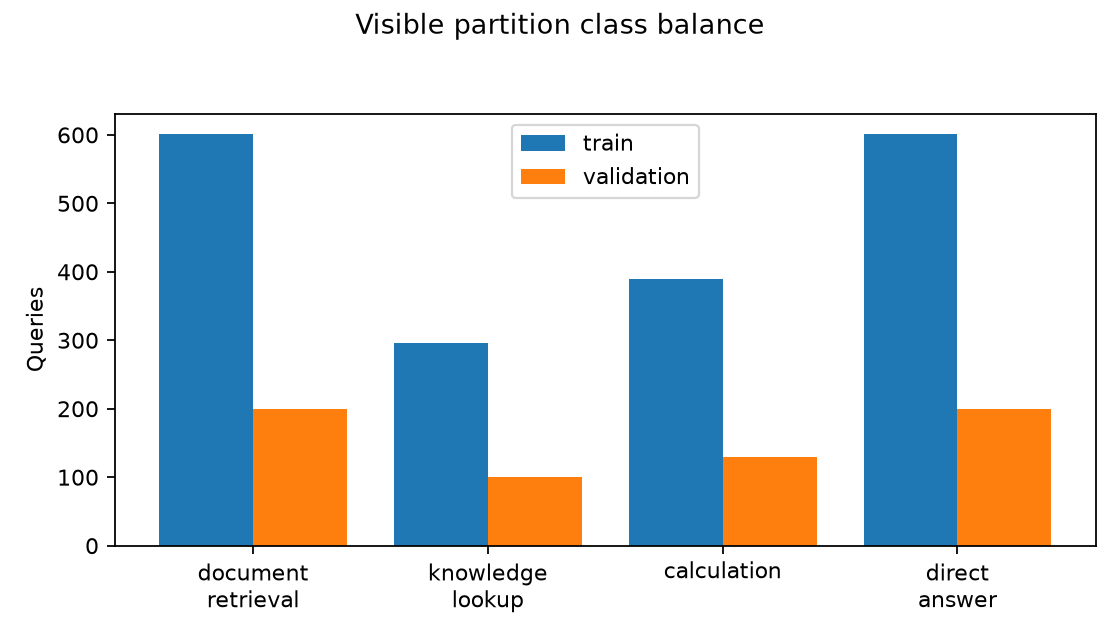
\includegraphics[width=\columnwidth]{figures/class-balance.png}
\caption{Training and validation support by first action. Lookup has 296
training and 100 validation examples. Macro-F1 gives it the same weight as
each of the larger classes.}\label{fig:balance}
\end{figure}
\begin{figure}[htbp]
\centering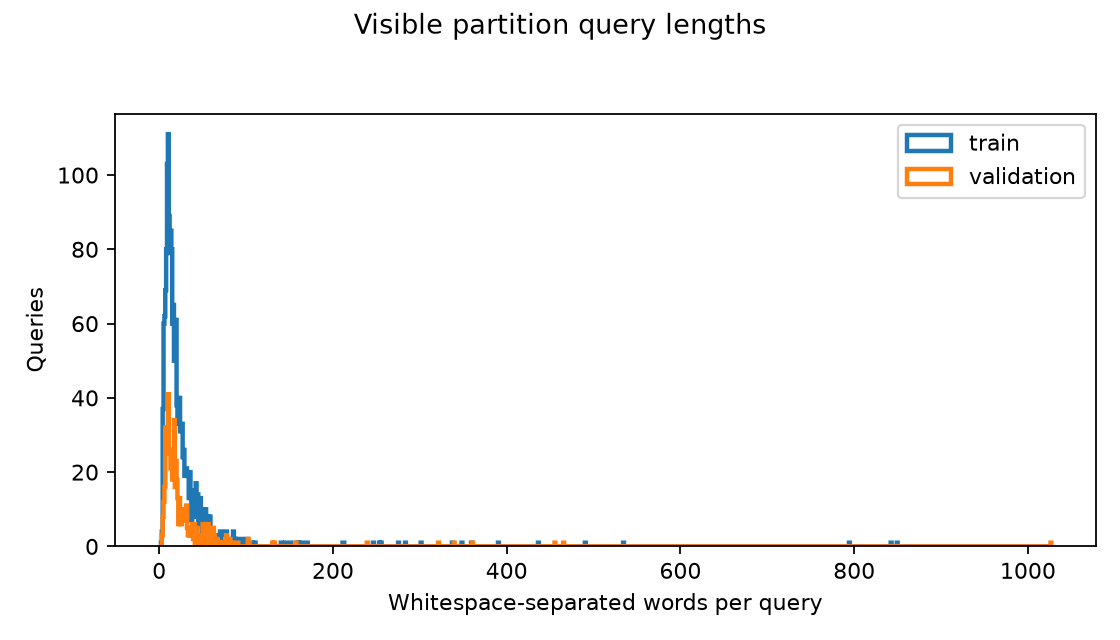
\includegraphics[width=\columnwidth]{figures/word-lengths.png}
\caption{Training and validation query lengths. Most queries cluster at the
short end, while a few extend into hundreds of words. Discuss how keeping some
passages inline could create a length cue. Its effect on predictions is unmeasured.}
\label{fig:length}
\end{figure}

\section{Methods and selection (1.5 pages)}
Explain the 26 local configurations. Start with the majority baseline and
multinomial naive Bayes on counts. Compare logistic regression on unigram counts
(L1), unigram TF-IDF (L2), and unigram plus bigram TF-IDF (L3). Compare L2 to
a linear SVM (S1) on the same features. Fit vocabulary and weights on training
rows alone. Describe the unigram TF-IDF decision tree, random forest and
XGBoost grids. Cite the frozen configuration for all settings.
Treat the 27th configuration, TypeSafe Jev 1.14.0, separately: it receives the
query and fixed action definitions and uses external pretraining.

Define macro-F1 as the unweighted mean of the four class F1 scores. Report
accuracy, class support and per-class scores alongside it. Explain the inclusive
0.01 validation macro-F1 tolerance and the predetermined within-family and
overall tie rules. Freeze the selected systems, calibration procedure and
threshold before describing the single test opening.

\section{Results (1.5 pages)}
Use Table~\ref{tab:results} for the frozen family winners. Explain why validation
selected Jev and why the local ordering changes on test. For a controlled feature
comparison, hold logistic regression and $C$ fixed: at $C=10$ adding bigrams
raises validation macro-F1 from 0.9324 to 0.9524, while at $C=0.1$ it lowers
it from 0.7345 to 0.7043. Compare counts versus TF-IDF and logistic versus SVM
at matched $C$ in the saved comparison. Separate API network timing from offline
replay timing when discussing cost.

\begin{table}[htbp]
\caption{Macro-F1 on 629 validation and 628 test queries. Selection used
validation. The test column reports the frozen configurations.}
\label{tab:results}\centering
\begin{tabular}{lrr}\toprule
System & Validation & Test \\ \midrule
B0 majority & 0.121 & 0.120 \\
B1 naive Bayes & 0.878 & 0.863 \\
L1-C1 & 0.922 & 0.896 \\
L2-C1 & 0.924 & 0.903 \\
S1-C1 & 0.936 & 0.945 \\
L3-C10 & 0.952 & 0.928 \\
DT-d30-leaf1 & 0.818 & 0.806 \\
RF-dNone-leaf1 & 0.913 & 0.900 \\
XGB-d6-lr0.05 & 0.901 & 0.871 \\
Jev (selected) & 0.975 & 0.964 \\ \bottomrule
\end{tabular}
\end{table}

\section{Confidence and errors (1.5 pages)}
Only L3-C10 received sigmoid calibration, fitted on three grouped training folds.
Compare its raw and calibrated test log loss (0.245 to 0.229), Brier score
(0.115 to 0.113) and five-bin ECE (0.087 to 0.055). Report bin sizes.
S1 supplies margins. Jev supplies its own probabilities. Explain coverage and
accuracy among accepted queries: at threshold 0.7 on validation, calibrated L3-C10
accepts 87.9\% at 98.4\% accuracy. Threshold 0.0 already met the 90\%
target at maximum coverage. Frozen on validation, it accepted all 628 test
queries at 93.2\% accuracy.

\begin{figure}[htbp]
\centering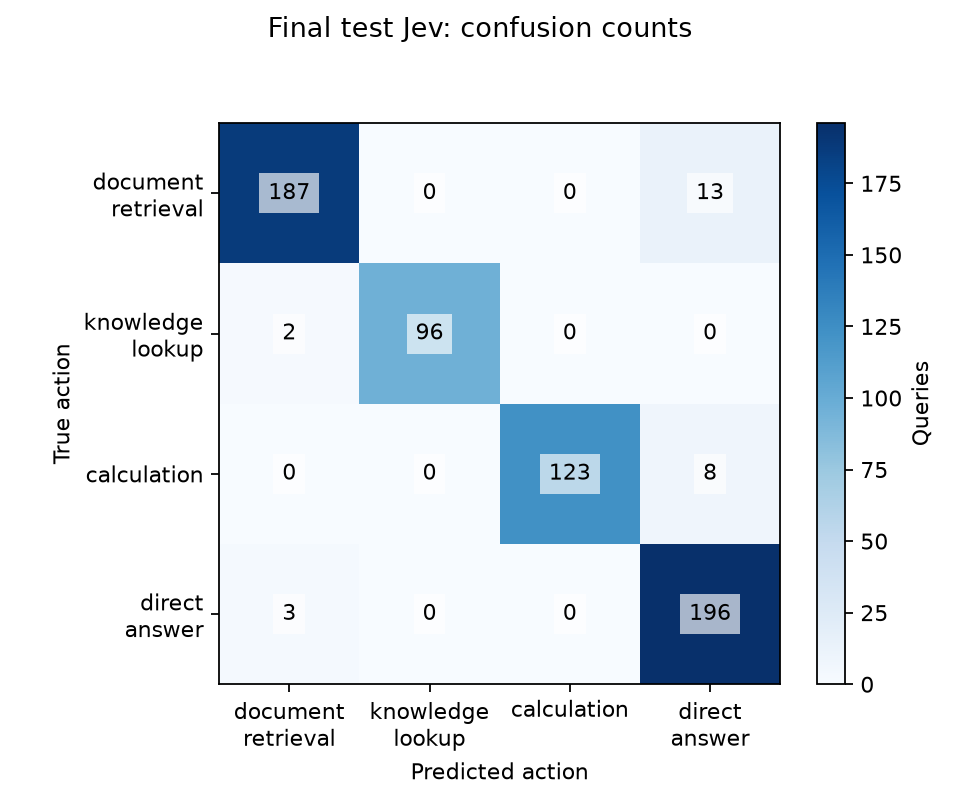
\includegraphics[width=\columnwidth]{figures/final-confusion-Jev.png}
\caption{Jev on the frozen test. Thirteen of its 26 errors sent a retrieval
query to direct answer. The denominator for retrieval recall is the 200
accepted retrieval labels in the first row.}\label{fig:errors}
\end{figure}
Use Fig.~\ref{fig:errors} to move from a count to a competing explanation.
Paraphrase q3014: the accepted label requires reading an attached passage, but
the router sees only a short summary request. Altan checked the attachment and
kept the label. Missing context is a hypothesis. Contrast a correct comparison
from the saved review ledger and a local error such as q2118, where L3-C10
predicted direct answer for a table lookup.

\section{Discussion and conclusion (0.5 page)}
Bound the findings to the release, its grouping rule and one test split.
Discuss shared AI label bias, corpus-specific phrasing, possible length cues
and unknown Jev pretraining overlap. Give the strongest supported conclusion
and propose one follow-up that could distinguish two explanations, such as a
future controlled comparison with and without an attachment indicator.

\section*{Reproducibility, assistance and references (0.5 page)}
Identify the dataset, split, run, freeze, receipt and archive using the evidence
map accompanying this outline. Distinguish the local rerun and Jev cache replay
from the two live validation passes, whose top choices differed on two rows.
Disclose agent assistance in data preparation, review, implementation and this
outline. In the draft, cite the dataset sources and licenses, methods and
implementation references actually used. Write the final account in your own words.
\end{document}
